\chapter{System Design and Architecture}\label{ch:architecture}

\section{Overall architecture}

Figure~\ref{fig:architecture} shows the components and their interactions. Three kinds of
clients use the database, each through a different account and access path:

\begin{itemize}
  \item The \textbf{billing application} (\code{TELCO\_APP}) writes and reads through the view
        \code{BILLING\_CURRENT\_V}. The view exposes only the hot months and rejects any row
        outside them.
  \item \textbf{Analysts and auditors} (\code{TELCO\_ANALYST}) read the whole retained history
        through \code{BILLING\_ALL}, the union of the online and archive tables.
  \item The \textbf{DBA or scheduler} (\code{TELCO\_OWNER}) runs the lifecycle package
        \code{DLM\_PKG}. The package reads its policy from \code{DLM\_CONFIG}, logs to
        \code{DLM\_JOB\_LOG} and validates against \code{BILLING\_CONTROL\_TOTALS}.
\end{itemize}

The benchmark harness runs in a separate tools container and reaches the database over TCP.
The baseline tables (\code{BILLING\_RECORDS\_BASE}, \code{BILLING\_ARCHIVE\_BASE}) live in the
same schema, so both designs are compared on the same server, data and workload.

\begin{sidewaysfigure}
  \centering
  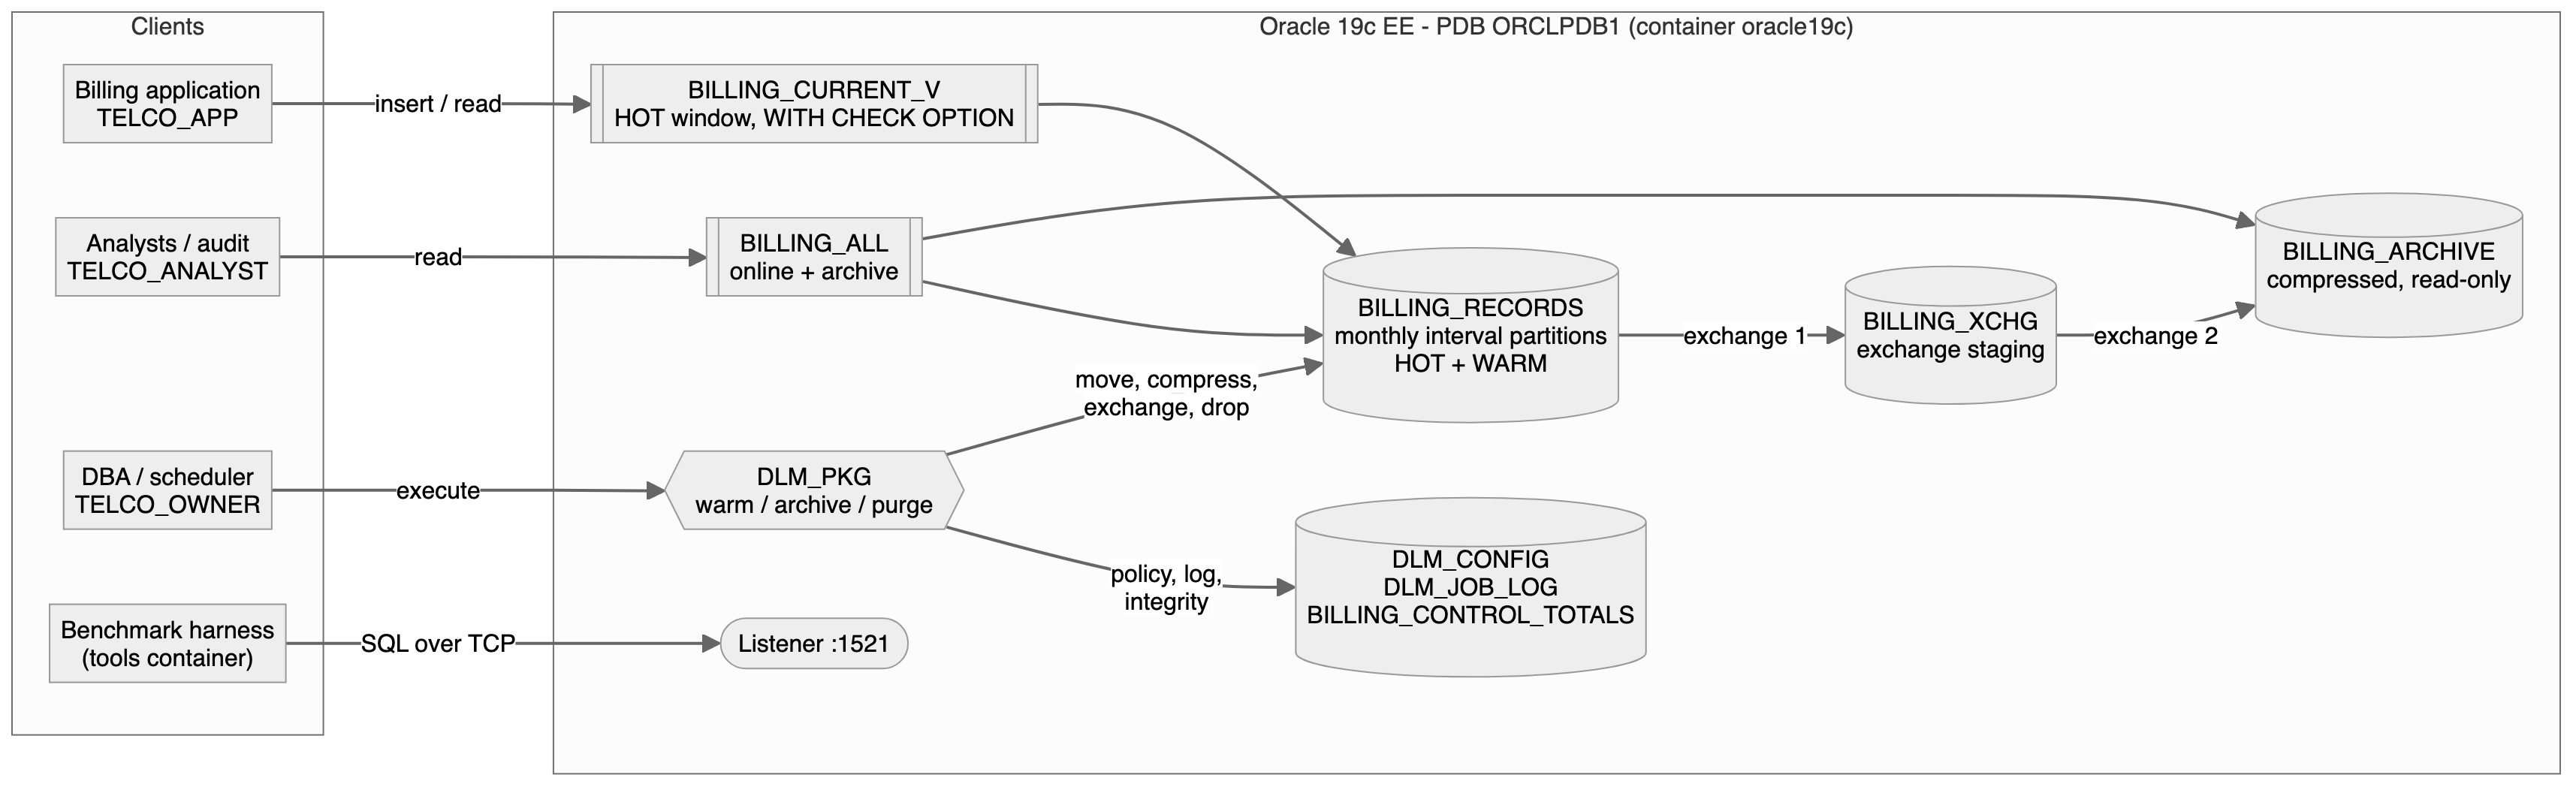
\includegraphics[width=\linewidth]{01_architecture}
  \caption{Overall system architecture}
  \label{fig:architecture}
\end{sidewaysfigure}

\section{Storage tiers and data lifecycle}

Each month moves through four states (Figure~\ref{fig:tiers}). Each state has its own
tablespace, storage format and access rights. Tablespaces separate the tiers physically:
\code{TELCO\_HOT} for current data, \code{TELCO\_IDX} for its indexes, and \code{TELCO\_ARCH}
for compressed warm and archived data. In production, \code{TELCO\_ARCH} could sit on cheaper
storage.

\begin{figure}[H]
  \centering
  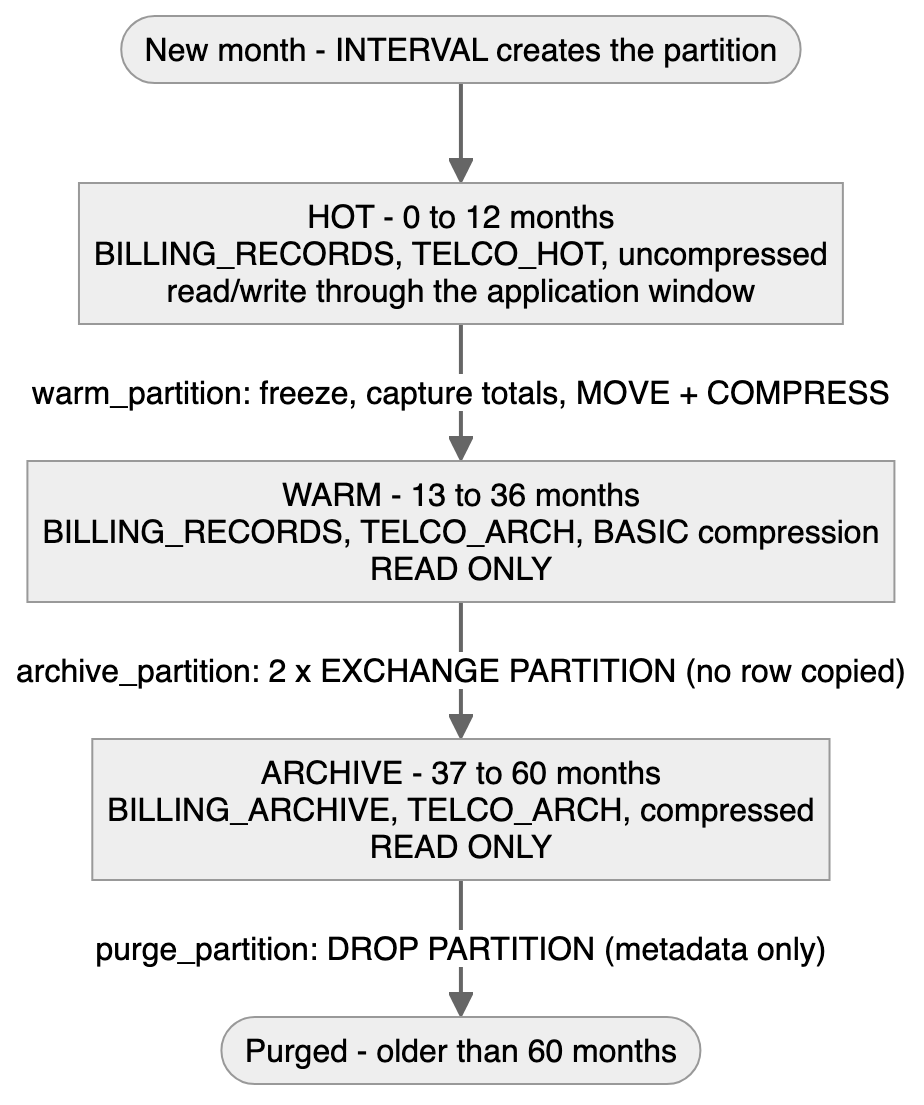
\includegraphics[width=0.62\linewidth]{02_tiers}
  \caption{Storage tiers and lifecycle operations}
  \label{fig:tiers}
\end{figure}

\begin{description}[style=nextline]
  \item[HOT (0--12 months)] Uncompressed in \code{TELCO\_HOT}. The application may insert
        late lines and corrections here through its window view.
  \item[WARM (13--36 months)] The month is \emph{frozen}: it is set read-only, its control
        totals are re-captured, and it is moved to \code{TELCO\_ARCH} with BASIC compression.
        It stays in \code{BILLING\_RECORDS}, so recent-history queries use the same table.
  \item[ARCHIVE (37--60 months)] The month leaves the online table for
        \code{BILLING\_ARCHIVE} through two partition exchanges, and stays compressed and
        read-only.
  \item[PURGED ($>$60 months)] The archive partition is dropped, which is a metadata operation.
\end{description}

\section{Archive sequence}

The key mechanism is the zero-copy archive (Figure~\ref{fig:sequence}). A partition can only
be exchanged with a non-partitioned table, so the month travels through the empty staging
table \code{BILLING\_XCHG}. Step~1 swaps the month's segment into the staging table. Step~2
creates the archive partition (\code{LOCK TABLE ... PARTITION FOR}) and swaps the segment into
it. Step~3 drops the now-empty online partition. No row is copied at any point. If the job
dies between steps 1 and 2, the data waits in \code{BILLING\_XCHG}: the integrity check
reports the month as missing, and the next run detects the staged rows and resumes at step~2.

\begin{sidewaysfigure}
  \centering
  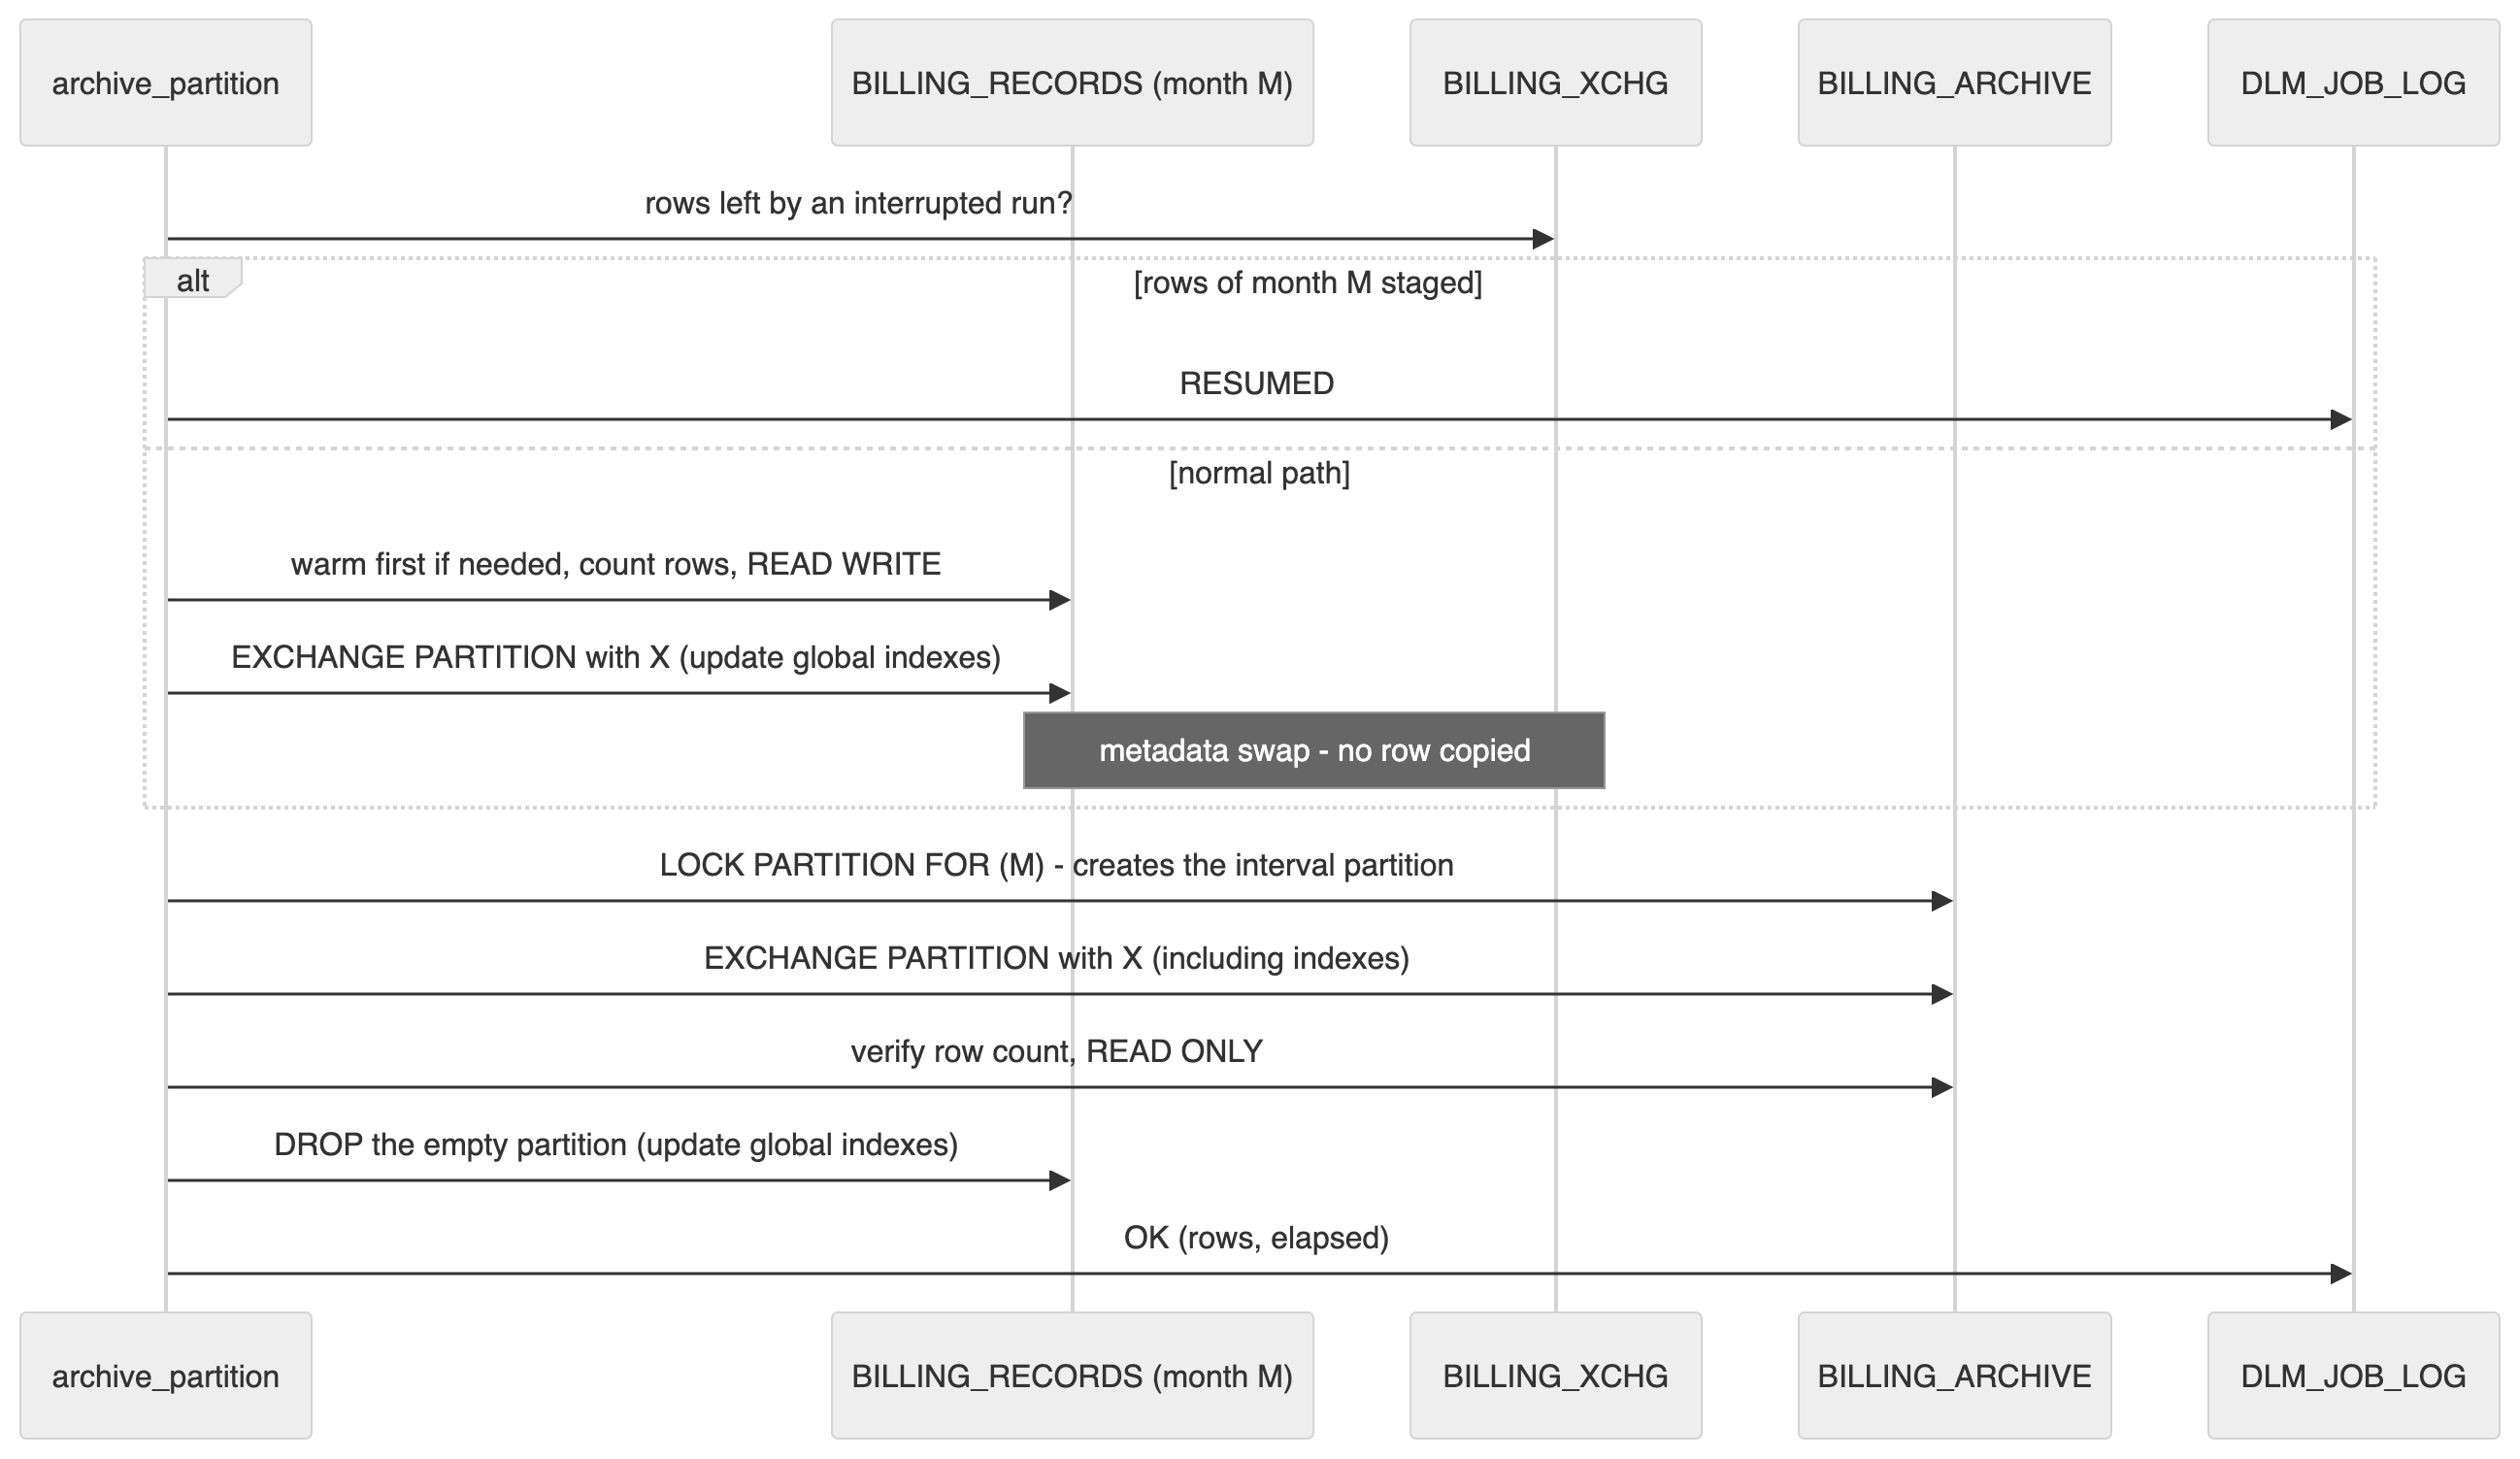
\includegraphics[width=0.95\linewidth]{03_archive_sequence}
  \caption{Archive of one month: sequence diagram}
  \label{fig:sequence}
\end{sidewaysfigure}

\section{Monthly job (activity)}

\code{run\_lifecycle} orchestrates a complete monthly run (Figure~\ref{fig:activity}). It
first closes the application window on the months it is about to freeze, then resumes any
interrupted archive, removes empty partitions left by rejected inserts, and re-applies
read-only on archive partitions. It then purges, warms and archives, refreshes incremental
statistics and validates every frozen month. If a frozen month differs from its control
totals, the job stops with \code{ORA-20040} so that an operator investigates.

\begin{figure}[H]
  \centering
  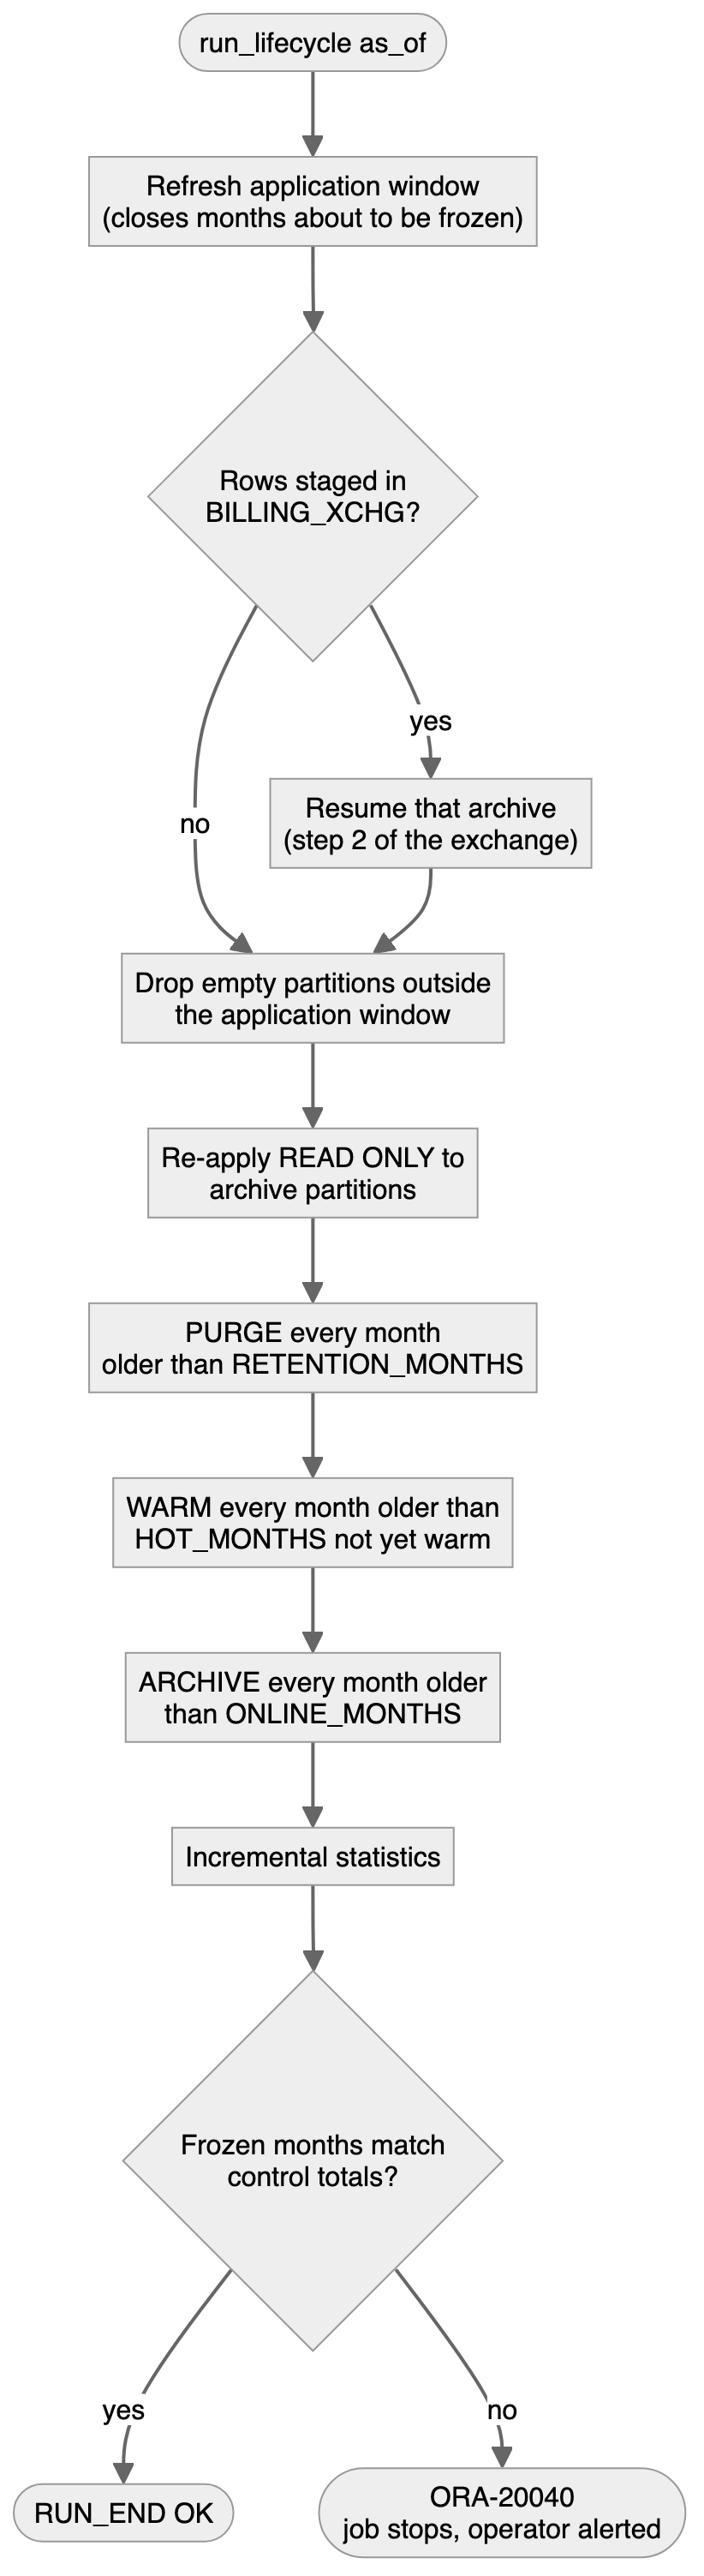
\includegraphics[height=0.72\textheight]{05_lifecycle_activity}
  \caption{Monthly lifecycle job: activity diagram}
  \label{fig:activity}
\end{figure}

\section{Logical data model}

\begin{figure}[H]
  \centering
  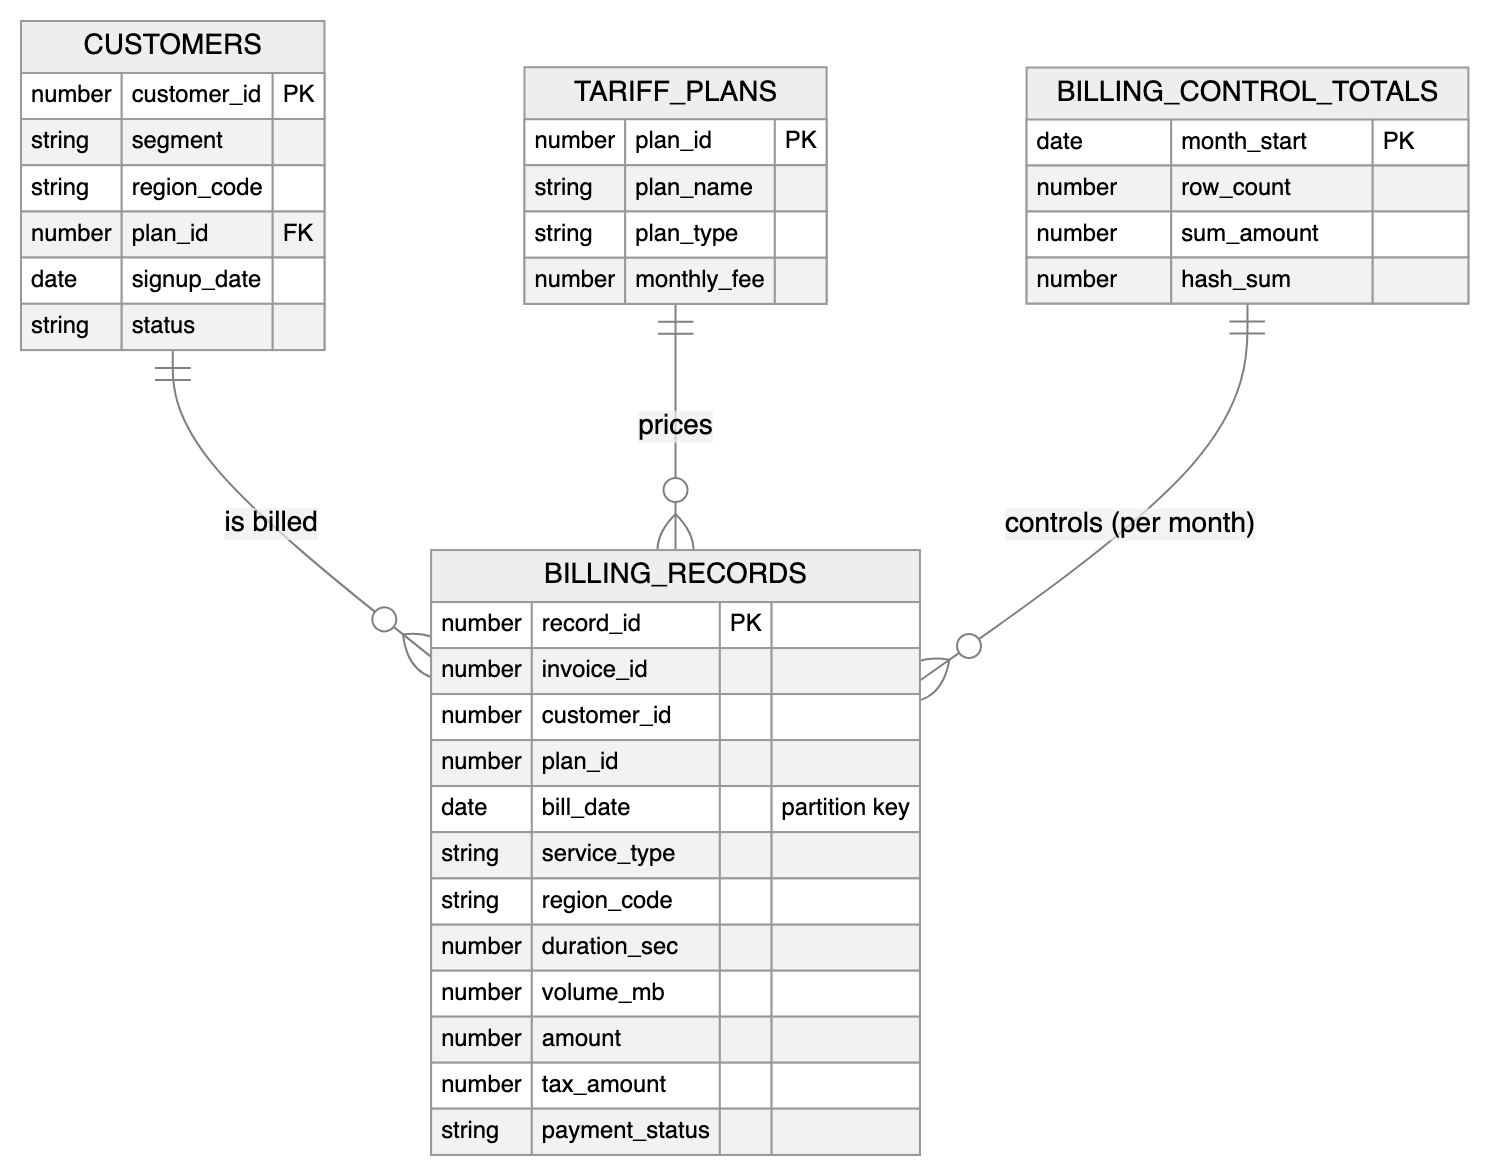
\includegraphics[width=0.85\linewidth]{04_data_model}
  \caption{Logical data model}
  \label{fig:datamodel}
\end{figure}

\code{BILLING\_RECORDS} is the fact table (one row per billed service line). Each customer
subscribes to one tariff plan (\code{CUSTOMERS.plan\_id}, foreign key), and the plan is copied
on every billing line. The other billing
tables (\code{BILLING\_ARCHIVE}, \code{BILLING\_XCHG}, the baseline tables and the load
staging table) are created from \code{BILLING\_RECORDS\_BASE} with
\code{CREATE TABLE ... AS SELECT ... WHERE 1=0}. This guarantees identical columns, which
partition exchange requires. The same \code{CHECK} constraints (service type, payment status,
non-negative amounts) are added to every billing table. There is no foreign key from the fact
table to \code{CUSTOMERS}: as in most billing and warehouse designs, the loading process
guarantees referential integrity, and a foreign key would complicate exchanges and slow bulk
loads.

\section{Indexing strategy}

\begin{table}[H]
\centering
\caption{Indexes of both designs}
\begin{tabularx}{\linewidth}{lllL}
\toprule
Design & Columns & Type & Purpose \\
\midrule
Baseline & \code{record\_id} & PK, B-tree & OLTP lookup \\
Baseline & \code{(customer\_id, bill\_date)} & B-tree & customer history \\
Baseline & \code{bill\_date} & B-tree & date-range reports \\
Partitioned & \code{record\_id} & PK, \textbf{global} B-tree & single probe for any online month \\
Partitioned & \code{(customer\_id, bill\_date)} & \textbf{local} B-tree & one segment per month, moves with it \\
Partitioned & \emph{none on} \code{bill\_date} & -- & replaced by partition pruning \\
Archive & \code{(customer\_id, bill\_date)} & local B-tree & swapped in by \code{INCLUDING INDEXES} \\
\bottomrule
\end{tabularx}
\end{table}

The main trade-off is the global primary key. It keeps lookups by \code{record\_id} to a single
probe, but it must be maintained (\code{UPDATE GLOBAL INDEXES}) whenever a partition is moved
or exchanged out. A local unique index must contain the partition key (ORA-14039), so the
alternative would be a local primary key on \code{(record\_id, bill\_date)}. Lifecycle
operations would then be pure metadata, but \code{record\_id} alone would no longer be
guaranteed unique, and lookups by \code{record\_id} would probe every partition.

\section{Security architecture}

\begin{table}[H]
\centering
\caption{Accounts and privileges (least privilege)}
\begin{tabularx}{\linewidth}{lLL}
\toprule
Account & Privileges & Cannot \\
\midrule
\code{TELCO\_OWNER} & owns the objects, runs DLM, \code{SELECT} on a few \code{V\$} views for benchmarking & -- (would be locked in production, with the job run by a scheduler) \\
\code{TELCO\_APP} & \code{INSERT}, \code{READ} on \code{BILLING\_CURRENT\_V}; \code{READ} on reference data & write outside the hot window, touch base tables, update or delete, read the archive or the policy, run DLM, DDL \\
\code{TELCO\_ANALYST} & \code{READ} on \code{BILLING\_ALL} and reference data & modify anything, lock tables, access base tables, policy or DLM \\
\bottomrule
\end{tabularx}
\end{table}

The other security measures are:

\begin{itemize}
  \item \textbf{No credentials in code or in Git.} A git-ignored \code{.env} (mode 600) is
        generated with random passwords. Passwords are sent to SQL*Plus through standard
        input, so they never appear in the process list. They are only used in
        \code{CREATE/ALTER USER} statements, which Oracle does not keep in clear text in
        \code{V\$SQL}.
  \item \textbf{\code{READ} instead of \code{SELECT}} for read-only accounts. With
        \code{SELECT}, an account can \code{LOCK TABLE} a view and block the lifecycle job; we
        verified this on the database. \code{READ} prevents it.
  \item \textbf{Frozen data is read-only} (ORA-14466 on any change). The application window
        rejects late rows in old months (ORA-01402).
  \item \textbf{Guards and audit trail.} Purges inside the legal retention are refused, and
        every action, refusal and error is logged.
\end{itemize}
